\documentclass{standalone}
\usepackage{tikz}
\usepackage{ctex,siunitx,ninecolors}
\setCJKmainfont{Noto Serif CJK SC}
\usepackage{tkz-euclide}
\usepackage{amsmath}
\usepackage{wasysym}
\usetikzlibrary{patterns, calc}
\usetikzlibrary{decorations.pathmorphing, decorations.pathreplacing, decorations.shapes,3d}
\begin{document}
\small
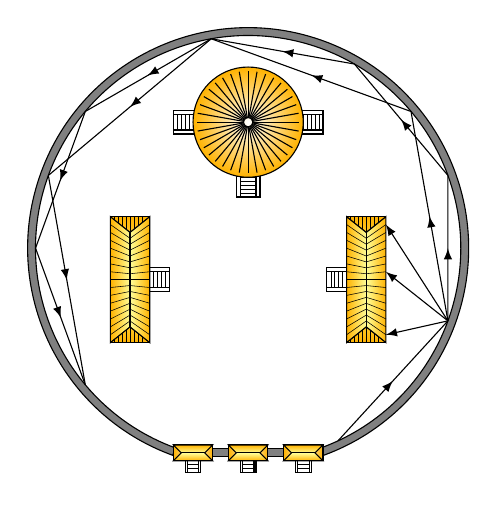
\begin{tikzpicture}[>=latex,scale=1.0]
  \useasboundingbox(-2.8,2.8)rectangle(2.8,-2.9);
  \draw[fill=gray](250:2.8)arc(250:-70:2.8)--++(110:0.1)arc(-70:250:2.7)--cycle;
  \foreach \x in {-0.9,-0.85,...,0.9}
  {
    \draw[very thin](\x,1.7)--++(0,-0.2);
  }
  \draw(-0.95,1.45)rectangle(0.95,1.75)(-0.95,1.5)rectangle(0.95,1.7);
  \foreach \x in {0.7,0.75,...,1.0}
  {
    \draw[very thin](-0.1,\x)--(0.1,\x);
  }
  \draw(-0.15,0.65)rectangle(0.15,1.0)(-0.1,0.65)rectangle(0.1,1.0);
  \draw[outer color=yellow!40!orange,inner color=white](0,1.6)circle(0.7);
  \foreach \x in {0,10,...,350}{ \draw([shift=(\x:0.05)]0,1.6)--++(\x:0.6);}
  \foreach \x in {1.05,1.1,...,1.3}
  {
    \draw[very thin](\x,-0.3)--(\x,-0.5);
    \draw[very thin](-\x,-0.3)--(-\x,-0.5);
  }
  \draw(-1.3,-0.3)rectangle(-1,-0.5)(1.3,-0.3)rectangle(1,-0.5);
  \draw(-1.3,-0.25)rectangle(-1,-0.55)(1.3,-0.25)rectangle(1,-0.55);
  \foreach \x in {-1.5,1.5}
  {
    \draw[top color=yellow!40!orange,bottom color=yellow!40!orange,middle color=yellow!40](\x-0.25,0.4)rectangle(\x+0.25,-1.2);
    \foreach \y in {-0.2,-0.15,...,0.2}{\draw[very thin](\x+\y,0.4)--(\x+\y,-1.2);}
    \draw[left color=yellow!40!orange,right color=yellow!40!orange,middle color=yellow!40](\x-0.25,0.4)--(\x-0.25,-1.2)--(\x,-1.0)--(\x+0.25,-1.2)--(\x+0.25,0.4)--(\x,0.2)--cycle;
    \draw(\x,0.2)--(\x,-1.0);
    \foreach \y in {-8,-7,...,8}
    {
      \draw[very thin] (\x,-0.4+\y*0.075)--(\x+0.25,-0.4+\y*0.1);
      \draw[very thin] (\x,-0.4+\y*0.075)--(\x-0.25,-0.4+\y*0.1);
    }
  }
  \draw[postaction={decorate},decoration={markings,mark=between positions 0.125 and 0.9 step 0.25 with {\arrow{>}} }](-20:2.7)\foreach \x in {40,100,...,260}{--(\x:2.7)};
  \draw[postaction={decorate},decoration={markings,mark=between positions 0.0833 and 0.92 step 0.167 with {\arrow{>}} }](-20:2.7)\foreach \x in {20,60,...,220}{--(\x:2.7)};
  \draw[postaction={decorate},decoration={markings,mark=at position 0.5 with {\arrow{>}} }](-65:2.7)--(-20:2.7);
  \draw[->](-20:2.7)--(1.75,-1.1);
  \draw[->](-20:2.7)--(1.75,-0.3);
  \draw[->](-20:2.7)--(1.75,0.3);
  \draw[fill=gray](-0.9,-2.65)rectangle(0.9,-2.55);
  \foreach \x in {-0.7,0,0.7}
  {
    \foreach \y in {-2.8,-2.75,...,-2.6}
    {
      \draw[very thin](\x-0.075,\y)--(\x+0.075,\y);
    }
    \draw(\x-0.075,-2.85)rectangle(\x+0.075,-2.6);
    \draw(\x-0.1,-2.85)rectangle(\x+0.1,-2.6);
    \draw[left color=yellow!40!orange,right color=yellow!40!orange,middle color=white](\x-0.25,-2.7)rectangle(\x+0.25,-2.5);
    \draw[top color=yellow!40!orange,bottom color=yellow!40!orange,middle color=yellow!40](\x-0.25,-2.7)--(\x+0.25,-2.7)--(\x+0.15,-2.6)--(\x+0.25,-2.5)--(\x-0.25,-2.5)--(\x-0.15,-2.6)--cycle;
    \draw(\x-0.15,-2.6)--(\x+0.15,-2.6);
    
  }
\end{tikzpicture}
\end{document}